\documentclass[12pt]{article}
\usepackage{amsmath}
\usepackage{multirow}
\usepackage{enumerate}
\usepackage{graphicx}
\usepackage{changepage}
\usepackage[all]{xy}
\usepackage{tikz}
\usetikzlibrary{shapes}

\setlength{\voffset}{-3cm}
\setlength{\hoffset}{-2cm}
\setlength{\parindent}{0cm}
\setlength{\textheight}{27cm}
\setlength{\textwidth}{17cm}


\begin{document}

\quad\\[2cm]

\begin{center}
{\Huge Statistics for Computing MA4413\\[0.8cm]
Midterm Examination 2\\[1cm]
{\bf Type B}}\\[2cm]
\end{center}

\begin{itemize}\itemsep0.6cm
\item Do not turn over the page until instructed to do so.
\item Rough work pages are provided within.
\item Useful formulae and statistical tables are provided at the back.
\item {\bf Enter your answers (using an ``X'') in the table on the last page.}
\item There are 15 questions in total: each correct answer = 1\% (\emph{there are no negative marks}).
\item For each question, only \emph{one} answer is correct.
\item Scientific calculators approved by the University of Limerick can be used.
\end{itemize}

\newpage
\section*{Questions 1 - 5}


\rule{\linewidth}{1pt}
\quad\\
Let $X \sim \text{Normal}(\mu=15,\sigma=4)$.\\[0.2cm]

{\bf Q1} What is the value of $\Pr(X > 19.2)$? {\footnotesize(rounded to 2 decimal places)}\\[0.2cm]
\begin{tabular}{cccc}
{\bf(a)} $0.07$ & {\bf(b)} $0.44$ & {\bf(c)} $1.05$  & {\bf(d)} $0.15$ \\[0.6cm]
\end{tabular}

{\bf Q2} In a group of size $n=40$, what is the value of $\Pr(\,\overline{\!X} > 14.7)$? {\footnotesize(rounded to 2 decimal places)}\\[0.2cm]
\begin{tabular}{cccc}
{\bf(a)} $0.53$ & {\bf(b)} $0.68$ & {\bf(c)} $0.32$ & {\bf(d)} $0.47$  \\[0.6cm]
\end{tabular}

%Let $X_1 \sim \text{Normal}(\mu_1=10,\sigma=4)$ and $X_2 \sim \text{Normal}(\mu_2=8,\sigma=3)$.\\[0.2cm]
%
%{\bf Q10} What is the value of $\Pr(X_1-X_2 < 0)$? {\footnotesize(rounded to 2 decimal places)}\\[0.2cm]
%\begin{tabular}{cccc}
%{\bf(a)} 0.40 & {\bf(b)} 0.34 & {\bf(c)} 0.66 & {\bf(d)} 0.60 \\[0.6cm]
%\end{tabular}


\rule{\linewidth}{1pt}
\quad\\
A particular Android app has 10,000 users overall. The developers think that at least 70\% of these users like a new feature. To investigate this claim, 600 users are contacted: 400 \mbox{respond} and it is found that 350 of them like the new feature.
\\[0.2cm]

{\bf Q3} What is the value of the statistic here?\\[0.2cm]
\begin{tabular}{cccc}
{\bf(a)} $0.035$  & {\bf(b)} $0.875$ & {\bf(c)} $0.583$ & {\bf(d)} $0.667$ \\[0.6cm]
\end{tabular}

{\bf Q4} What is the parameter here? \\[0.2cm]
\begin{tabular}{cccc}
{\bf(a)} $\mu=$ unknown & {\bf(b)}  $p=$ 0.7 & {\bf(c)} $p=$ unknown & {\bf(d)} $\mu=$ 70 \\[0.6cm]
\end{tabular}



\rule{\linewidth}{1pt}

\quad\\
Consider the following sample of ages of computers in an office block:
\begin{center}
\begin{tabular}{|ccc|}
\hline
&&\\[-0.3cm]
4.3 & 5.1 & 2.6 \\[0.1cm]
\hline
\end{tabular}
\end{center}
{\bf Q5} The 95\% confidence interval for the mean is:\\[0.2cm]
\begin{tabular}{cccc}
{\bf(a)} $[1.85,\,\,6.15]$ & {\bf(b)} $[0.83,\,\,7.17]$ & {\bf(c)} $[2.56,\,\,5.44]$ & {\bf(d)} $[1.65,\,\,6.35]$ \\[0.6cm]
\end{tabular}

\quad

\rule{\linewidth}{1pt}

\newpage

\section*{Rough Work\\[23cm]}
\section*{\hspace{8cm}$\boxed{\text{Next page: Questions 6 - 10}}$}

\newpage


\section*{Questions 6 - 10}


\rule{\linewidth}{1pt}
\quad\\
{\bf Q6} Identify the statement that is \emph{false} (note: only one is false).\\[0.2cm]
%{\footnotesize(answer is given to two decimal places)}\\[0.2cm]
\begin{tabular}{c@{\,\,\,}llll}
{\bf(a)} & The standard error tends to increase as the sample size increases.\\[0.2cm]
{\bf(b)} & The population mean does not vary from sample to sample. \\[0.2cm]
{\bf(c)} & Increasing the confidence level leads to an increase in the confidence interval width. \\[0.2cm]
{\bf(d)} & The sample mean varies from sample to sample. \\[0.6cm]
\end{tabular}


\rule{\linewidth}{1pt}
\quad

On average, potholes arise on a road at a rate of 2 per mile according to a Poisson distribution.\\[0.2cm]

{\bf Q7} What is the probability that there are 3 potholes on a 2 mile stretch of road?\\[0.2cm]
\begin{tabular}{cccc}
{\bf(a)} $0.1954$ & {\bf(b)} $0.1804$  & {\bf(c)} $0.7619$& {\bf(d)} $0.3233$ \\[0.6cm]
\end{tabular}

{\bf Q8} What is the average distance (in miles) between potholes?\\[0.2cm]
\begin{tabular}{cccc}
{\bf(a)} $\frac{1}{4}$ & {\bf(b)} $4$ & {\bf(c)} $\frac{1}{2}$ & {\bf(d)} $2$ \\[0.6cm]
\end{tabular}

\rule{\linewidth}{1pt}
\quad\\
The lifetime of a particular component has an exponential distribution (i.e., $T \sim \text{Exponential}(\lambda)$) with an average life of 6 months.\\[0.3cm]
{\bf Q9} What is the probability that the component lasts more than 12 months? \\[0.2cm]
\begin{tabular}{cccc}
{\bf(a)} 0.1353 & {\bf(b)} 0.0088 & {\bf(c)} 0.0025 & {\bf(d)} 0.1146\\[0.6cm]
\end{tabular}

{\bf Q10} Let $T_1$ and $T_2$ represent the lifetimes for two of the components described above. Assuming these components work/fail independently, what is $\Pr(T_1 < 12 \cup T_2 < 12)$? \\[0.2cm]
\begin{tabular}{cccc}
{\bf(a)} $0.7477$ & {\bf(b)} $0.8647$ & {\bf(c)} $0.9817$  & {\bf(d)} $0.0183$ \\[0.6cm]
\end{tabular}

\rule{\linewidth}{1pt}

\newpage

\section*{Rough Work\\[23cm]}
\section*{\hspace{8cm}$\boxed{\text{Next page: Questions 11 - 15}}$}

\newpage

\section*{Questions 11 - 15}

\rule{\linewidth}{1pt}
\quad\\
Consider an $M/M/1$ system where the arrival rate is 8/hour and the service rate is 12/hour.\\[0.2cm]

{\bf Q11} On average, how long (in hours) does a customer spend in this system?\\[0.2cm]
\begin{tabular}{cccc}
{\bf(a)} $0.667$ & {\bf(b)} $0.250$ & {\bf(c)} $0.050$ & {\bf(d)} $4.00$ \\[0.6cm]
\end{tabular}

{\bf Q12} On average, how many customers are in the \emph{queue} component?\\[0.2cm]
\begin{tabular}{cccc}
{\bf(a)} $2.00$ & {\bf(b)} $0.167$ & {\bf(c)} $1.333$ & {\bf(d)} $0.667$ \\[0.6cm]
\end{tabular}


\rule{\linewidth}{1pt}
\quad\\
A manufacturer wants to compare two designs of CPU in terms of their typical operating temperature (degrees Celsius). Two small samples are selected and the results are as follows:
\begin{small}
\begin{center}
\begin{tabular}{|c|c|c|}
\hline
&&\\[-0.3cm]
& Design A & Design B \\
\hline
&&\\[-0.2cm]
sample size      & 6 & 8 \\[0.2cm]
mean   & 38.7 $^\circ$C & 30.1 $^\circ$C \\[0.2cm]
variance &  3.0 $^\circ$C$^2$ & 12.0 $^\circ$C$^2$ \\[0.2cm]
\hline
\multicolumn{3}{c}{}
\end{tabular}
\end{center}
\end{small}


{\bf Q13} If we wish to assume equal variances (i.e., $\sigma_1^2=\sigma_2^2$) when constructing a confidence interval for $\mu_1-\mu_2$, we must carry out the F-test first. In the case of the data shown above, what is the critical value for the F test? \\[0.2cm]
%{\footnotesize(hint: cannot use tables)}\\[0.2cm]
\begin{tabular}{cccc}
{\bf(a)} 5.60 & {\bf(b)} 5.29 & {\bf(c)} 4.00 & {\bf(d)} 6.85 \\[0.6cm]
\end{tabular}

{\bf Q14} If we choose \emph{not} to assume equal variances when constructing the confidence interval for $\mu_1-\mu_2$ here, what is the value of $\nu$ needed to look up the appropriate $t_{\,\nu,\,\alpha/2}$ value in the tables?\\[0.2cm]
%{\footnotesize(hint: use tables)}\\[0.2cm]
\begin{tabular}{cccc}
{\bf(a)} 11 & {\bf(b)} 12  & {\bf(c)} 13 & {\bf(d)} 14 \\[0.6cm]
\end{tabular}


\rule{\linewidth}{1pt}
\quad\\
A 99\% confidence interval for the average salary (in thousands) of a computer programmer was calculated as $[30.5,\,45.8]$.\\[0.2cm]

{\bf Q15} What does the ``\,99\%\,'' refer to?\\[0.4cm]
\begin{tabular}{c@{\,\,\,}llll}
\multicolumn{2}{l}{\quad The probability that:}\\[0.2cm]
{\bf(a)} & the average salary for our sample lies in the interval\,;\\[0.2cm]
{\bf(b)} & a randomly chosen programmer has a salary in the interval\,; \\[0.2cm]
{\bf(c)} & the average salary for the population lies in the interval\,; \\[0.2cm]
{\bf(d)} & a computer science student gets this question correct. \\[0.6cm]
\end{tabular}


\rule{\linewidth}{1pt}







\newpage

\section*{Rough Work\\[23cm]}
\section*{\hspace{2cm}$\boxed{\text{Don't forget to enter your answers on the last page!}}$}

\newpage


\section*{Useful Formulae: Page 1\\[0.3cm]}
{\bf Numerical Summaries:}\\[-0.8cm]
\begin{align*}
\bullet\quad \bar x &= \frac{\sum\,x_i}{n}\\[0.6cm]
\bullet\quad s^2 &= \frac{\sum\,x_i^2 - n\,\bar x^2}{n-1}\\
\end{align*}
{\bf Probability:}\\[-0.8cm]
\begin{align*}
\bullet\quad \Pr(A^c) &= 1 - \Pr(A) \\[1cm]
\bullet\quad \Pr(A \cup B) &= \Pr(A) + \Pr(B) - \Pr(A \cap B)\\[0.6cm]
\bullet\quad \Pr(E_1 \cup E_2 \cup \cdots \cup E_k) &= \Pr(E_1) + \Pr(E_2) + \cdots + \Pr(E_k) \text{\quad{\footnotesize(if mutually exclusive)}}\\[1cm]
\bullet\quad \Pr(A \cap B) &= \Pr(A) \, \Pr(B \, | \, A) = \Pr(B) \, \Pr(A \, | \, B) \\[0.6cm]
\bullet\quad \Pr(E_1 \cap E_2 \cap \cdots \cap E_k) &= \Pr(E_1) \, \Pr(E_2) \, \cdots \, \Pr(E_k) \text{\quad{\footnotesize(if independent)}}\\[1cm]
\bullet\quad \Pr(A\,|\,B) &= \frac{\Pr(A \cap B)}{\Pr(B)} = \frac{\Pr(A) \,\Pr(B\,|\,A)}{\Pr(B)}\\[1cm]
\bullet\quad \text{If $E_1,\ldots, E_k$} & \,\, \text{are mutually exclusive \& exhaustive}\\[0.1cm]
\Rightarrow \Pr(B) &= \Pr(B \cap E_1) + \Pr(B \cap E_2) + \cdots + \Pr(B \cap E_k) \\[0.2cm]
&= \Pr(E_1) \, \Pr(B\,|\,E_1) + \Pr(E_2) \, \Pr(B\,|\,E_2) + \cdots + \Pr(E_k) \, \Pr(B\,|\,E_k)\\
\end{align*}
{\bf Distributions:}\\[-0.8cm]
\begin{center}
\begin{tabular}{|c@{\qquad}|c@{\qquad}|c@{\qquad}|}
\hline
&&\\[-0.3cm]
$\bullet\quad X \sim \text{Poisson}(\lambda)$ & $\bullet\quad T \sim \text{Exponential}(\lambda)$ & $\bullet\quad X \sim \text{Normal}(\mu,\sigma)$ \\[0.6cm]
${\displaystyle\bullet\quad \Pr(X=x) = \frac{\lambda^x}{x\,!}\,\,e^{-\lambda}}$ & $\bullet\quad \Pr(T>t) = e^{-\lambda\,t}$ & ${\displaystyle\bullet\quad \Pr(X>x) = \Pr\left(Z > \frac{x-\mu}{\sigma}\right)}$\\[0.8cm]
$\bullet\quad x \in \{0,1,2,\ldots,\infty\}$ & $\bullet\quad t \in [0,\,\infty)$ & $\bullet\quad x \in (-\infty,\,\infty)$ \\[0.8cm]
$\bullet\quad E(X) = \lambda$ & ${\displaystyle\bullet\quad E(T) = \frac{1}{\lambda}}$ & $\bullet\quad E(X) = \mu$ \\[0.8cm]
$\bullet\quad Var(X) = \lambda$ & ${\displaystyle\bullet\quad Var(T) = \frac{1}{\lambda^2}}$ & $\bullet\quad Var(X) = \sigma^2$ \\[0.4cm]
\hline
\end{tabular}
\end{center}


\newpage

\section*{Useful Formulae: Page 2\\[0.3cm]}
{\bf Queueing Theory:}\\[-0.8cm]
\begin{align*}
\bullet\quad E(N) &= \lambda_a\,E(T)\\[0.6cm]
\bullet\quad \rho &= \frac{\lambda_a}{\lambda_s}\\[0.6cm]
\xymatrixcolsep{0.5cm}
\bullet\quad M/M/1 \text{ System:} \quad & \xymatrix{\lambda_a \ar@{->}[r] & \hspace{-0.1cm}
{\begin{tabular}{@{}c|@{}c|@{}c|@{}c|@{}c|@{}c}
\cline{1-5}
&&&& &
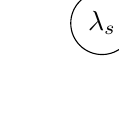
\begin{tikzpicture}[baseline=(char.base)]
\node(char)[draw,shape=circle]{$\lambda_s$};
\end{tikzpicture}\\
\cline{1-5}
\end{tabular}} \hspace{-0.3cm}\ar@{->}[r] &  \lambda_a} \\[0.6cm]
&\Rightarrow \,\, T \sim \text{Exponential}(\lambda_s-\lambda_a)\\[0.1cm]
{\footnotesize(\text{where $T$}} & {\footnotesize\text{ is the total time in the system)}}\\
\end{align*}

{\bf Normal Distribution:}\\[-0.8cm]
\begin{align*}
\bullet\quad \Pr(Z < -z) &= \Pr(Z > z) \\[0.6cm]
\bullet\quad \Pr(Z > -z) &= \Pr(Z < z) = 1 -\Pr(Z>z) \\[0.6cm]
\bullet\quad \Pr(X > x) &= \Pr\left(Z> \frac{x-\mu}{\sigma}\right)\\[0.6cm]
\bullet\quad (1-\alpha)100\% \text{ of the Normal}(\mu,\sigma) & \text{ distribution lies in } \mu \pm z_{\,\alpha/2}\,\,\sigma \\[1cm]
\bullet\quad \text{If} \,\,  X_1 \sim \text{Normal}(\mu_1,\sigma_1) \,\,  & \text{ and } \,\, X_2 \sim \text{Normal}(\mu_2,\sigma_2) \\[0.4cm]
\Rightarrow \quad  \text{ Sum: } \quad  X_1 + X_2 &\sim \text{Normal}\left(\mu_1+\mu_2,\,\sqrt{\sigma_1^2+\sigma_2^2}\,\right) \\[0.4cm]
\Rightarrow \quad  \text{ Difference: } \quad   X_1 - X_2 &\sim \text{Normal}\left(\mu_1-\mu_2,\,\sqrt{\sigma_1^2+\sigma_2^2}\,\right) \\[1cm]
\bullet\quad \text{For} \,\,  X_1,\ldots,X_n \sim \text{any distribution} & \text{ with } \mu = E(X) \text{ and } \sigma = Sd(X) = \sqrt{Var(X)}\\[0.4cm]
\Rightarrow \quad  \text{ Sample mean: } \quad  \,\overline{\!X} &\sim \text{Normal}\left(\mu,\,\frac{\sigma}{\sqrt{n}}\,\right) \quad \text{ if } n > 30
\end{align*}

\newpage


\section*{Useful Formulae: Page 3\\[0.3cm]}
{\bf Confidence Intervals:}\\[-0.8cm]
\begin{align*}
\bullet\quad \text{Large sample:} \qquad \text{statistic } &\pm\,\, z_{\,\alpha/2}\,\times\,\text{standard error} \\[0.6cm]
\bullet\quad \text{Small sample:} \qquad \text{statistic } &\pm\,\, t_{\,\nu,\,\alpha/2}\,\times\,\text{standard error}
\end{align*}
\begin{center}
\begin{tabular}{|c|c|c|c|c|}
\hline
&&&&\\[-0.1cm]
Parameter & Statistic & Standard Error & Samples & D. of. F. \\[0.3cm]
\hline
&&&&\\[-0.1cm]
$\mu$ & $\bar x$ & ${\displaystyle\frac{s}{\sqrt{n}}}$  & large / small & $\nu = n - 1$ \\[0.5cm]
\hline
&&&&\\[-0.1cm]
$p$ & $\hat p$ & \multirow{1}{*}{${\displaystyle\sqrt{\frac{\hat p\,(1-\hat p)}{n}}}$} & large & n/a \\[0.7cm]
\hline
&&&&\\[-0.1cm]
$\mu_1-\mu_2$ & $\bar x_1 - \bar x_2$ & \multirow{3}{*}{${\displaystyle\sqrt{\frac{s_1^2}{n_1}+\frac{s_2^2}{n_2}}}$} & large / small & ${\displaystyle \nu = \frac{(a+b)^2}{\frac{a^2}{n_1-1}+\frac{b^2}{n_2-1}}}$ \\[0.8cm]
&&&& ${\displaystyle a=\frac{s_1^2}{n_1}, \,\,\, b=\frac{s_2^2}{n_2}}$ \\[0.5cm]
\cline{3-5}
&&&&\\[-0.1cm]
&  & ${\displaystyle\sqrt{\frac{s_p^2}{n_1}+\frac{s_p^2}{n_2}}}$ & small & $\nu = n_1+n_2-2$ \\[0.5cm]
&&&& assuming \\[-0.2cm]
&& where\,\, ${\displaystyle s_p^2 = \frac{(n_1-1)\,s_1^2+(n_2-1)\,s_2^2}{n_1+n_2-2}}$  && $\sigma_1^2 = \sigma_2^2$ \\[0.5cm]
\hline
&&&&\\[-0.1cm]
$p_1-p_2$ & $\hat p_1 - \hat p_2$ & \multirow{2}{*}{${\displaystyle\sqrt{\frac{\hat p_1 \, (1-\hat p_1)}{n_1}+\frac{\hat p_2 \, (1-\hat p_2)}{n_2}}}$} & large & n/a\\[0.9cm]
\hline
\multicolumn{5}{c}{}\\[0.5cm]
\end{tabular}
\end{center}
\begin{align*}
\bullet\quad F &= \frac{\text{larger variance}}{\text{smaller variance}} = \frac{s_{\text{larger}}^2}{s_{\text{smaller}}^2} \\[0.3cm]
 & \nu_1 = \text{top sample size} - 1\\[0.1cm]
  & \nu_2 = \text{bottom sample size} - 1
\end{align*}



\newpage


\begin{adjustwidth}{-1cm}{0cm}
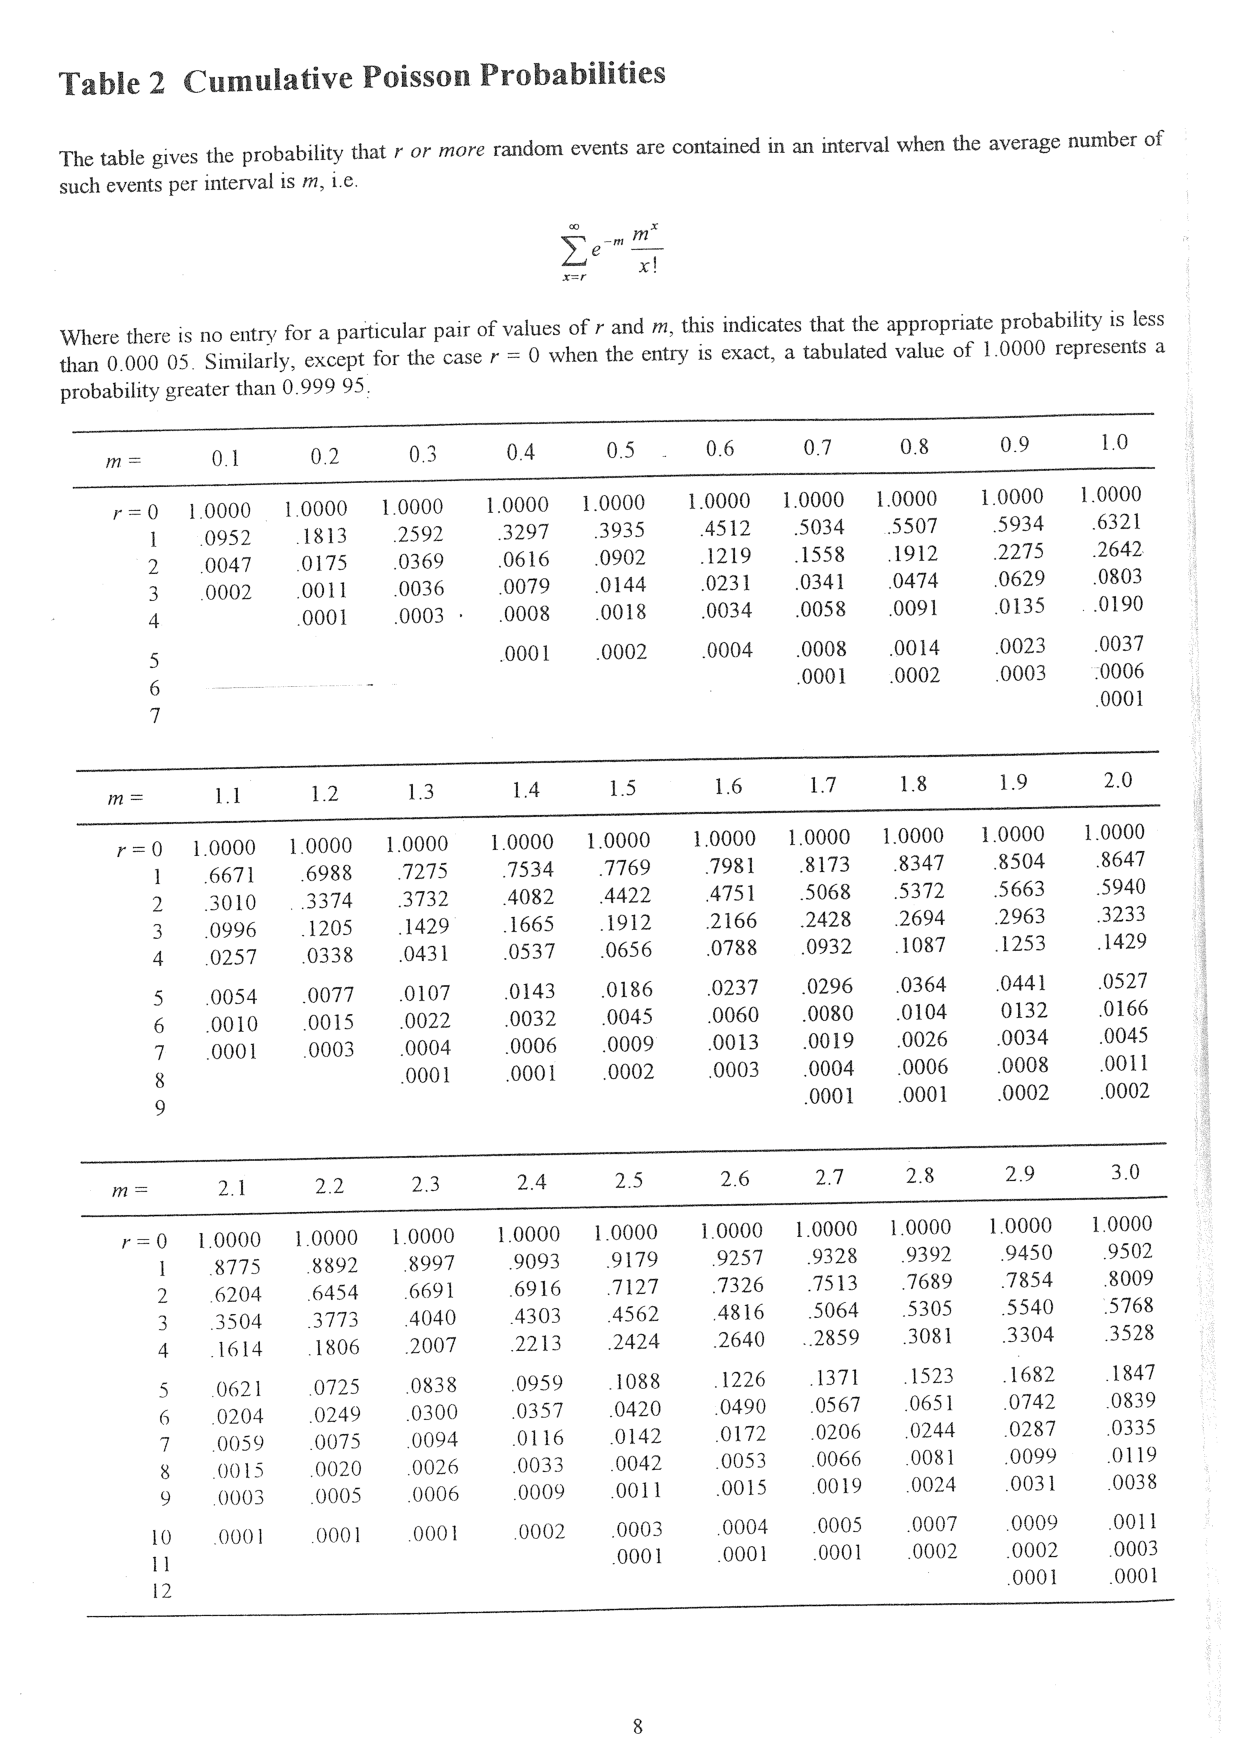
\includegraphics[width=1.1\textwidth, trim = 1cm 1cm 1cm 1cm, clip]{mdpois1}
\end{adjustwidth}

\newpage

\begin{adjustwidth}{-1cm}{0cm}
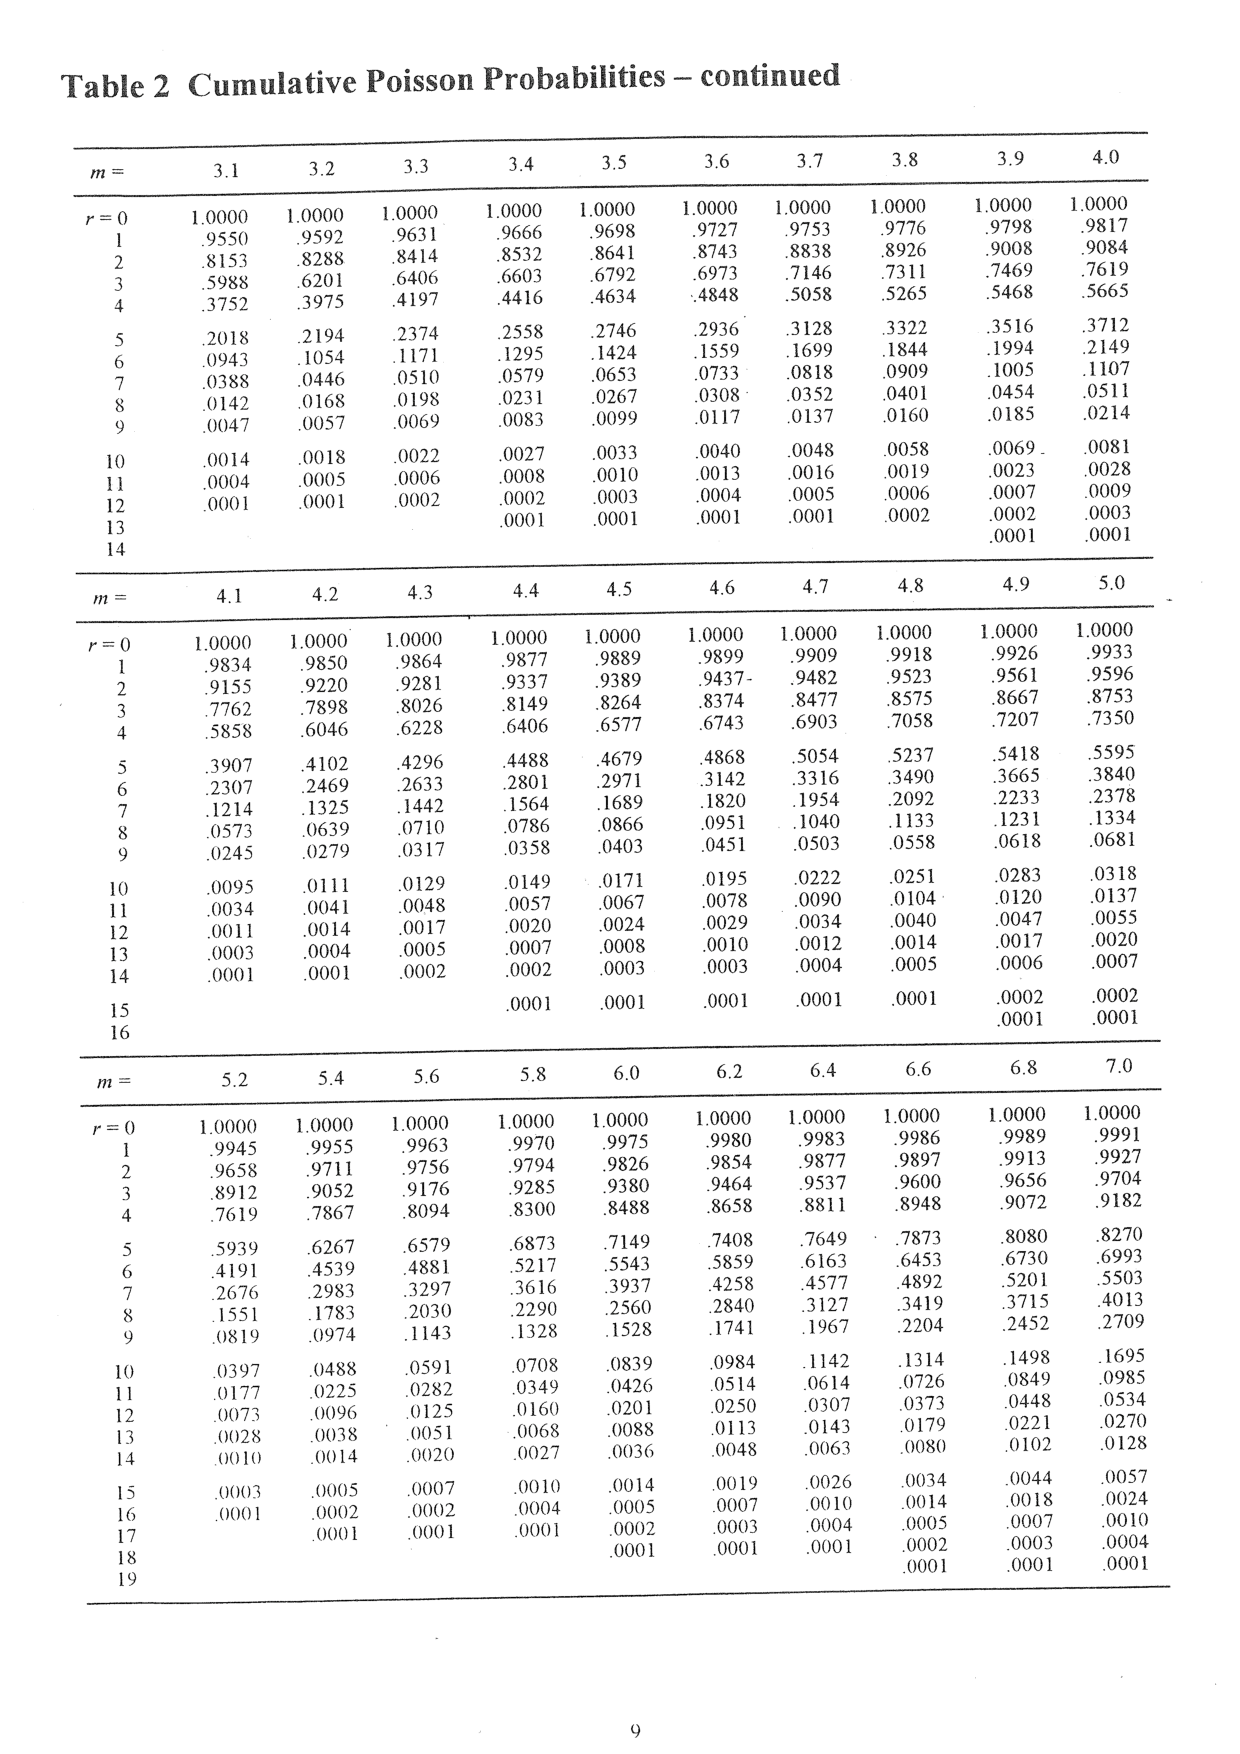
\includegraphics[width=1.1\textwidth, trim = 1cm 1cm 1cm 1cm, clip]{mdpois2}
\end{adjustwidth}

\newpage

\begin{adjustwidth}{-1cm}{0cm}
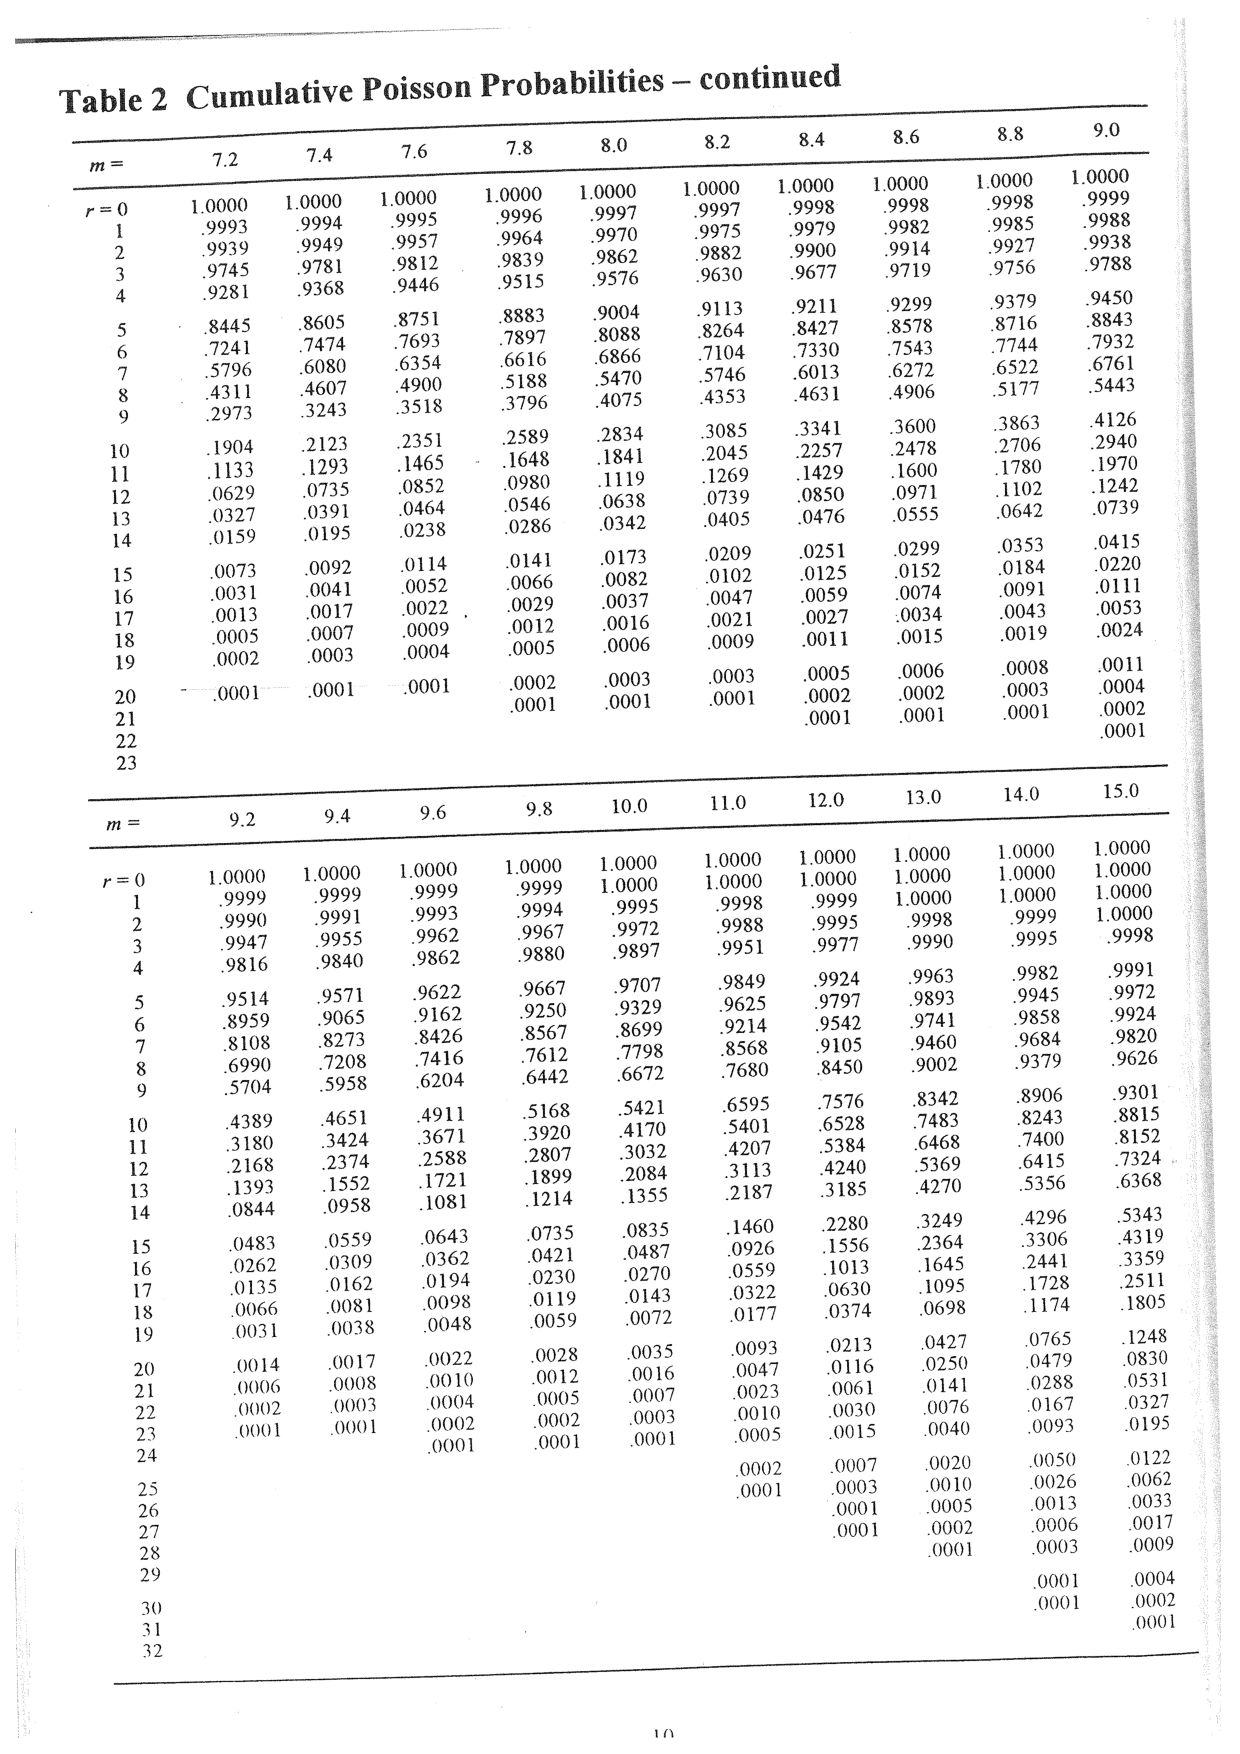
\includegraphics[width=1.1\textwidth, trim = 1cm 1cm 1cm 1cm, clip]{mdpois3}
\end{adjustwidth}

\newpage


\begin{adjustwidth}{-1cm}{0cm}
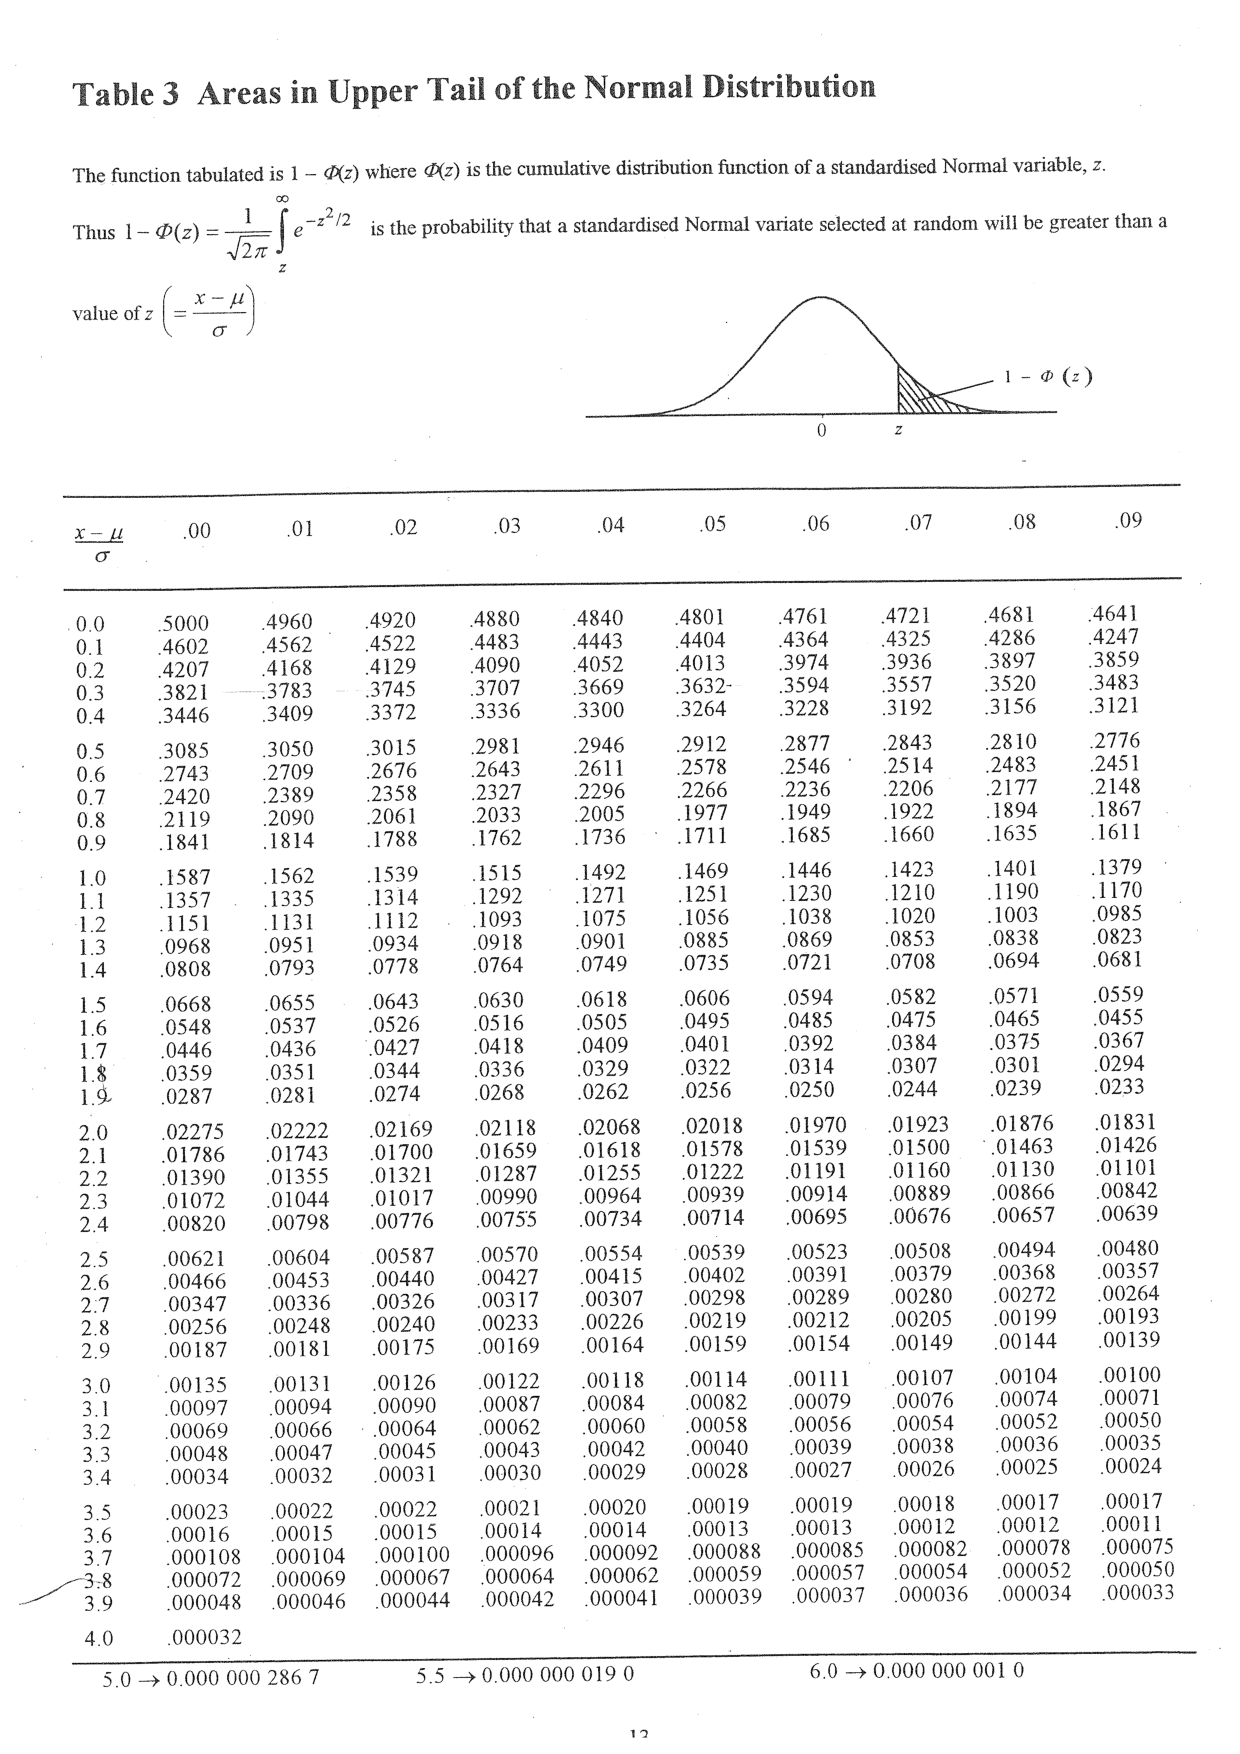
\includegraphics[width=1.1\textwidth, trim = 1cm 1cm 1cm 1cm, clip]{mdnorm}
\end{adjustwidth}

\newpage


\begin{adjustwidth}{-1cm}{0cm}
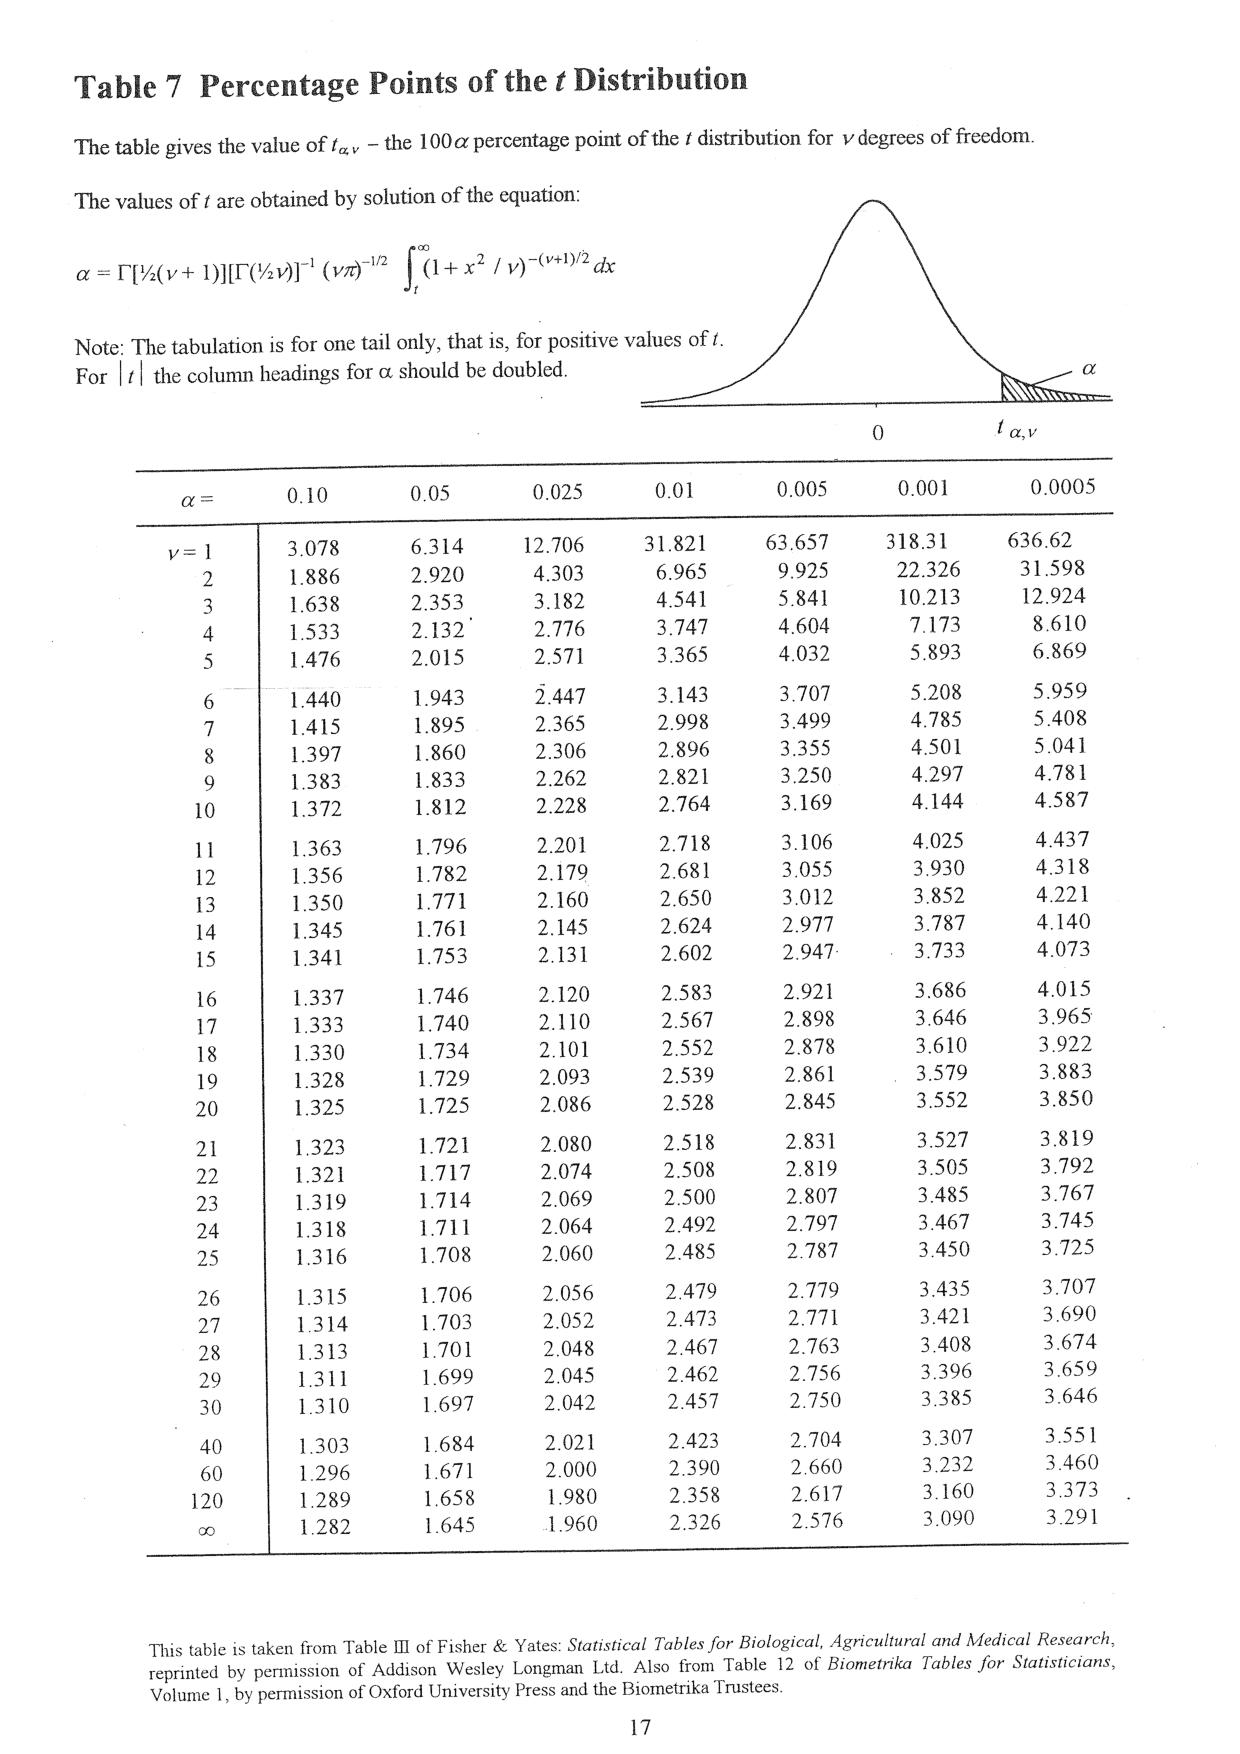
\includegraphics[width=1.1\textwidth, trim = 1cm 1cm 1cm 1cm, clip]{mdt}
\end{adjustwidth}

\newpage



\begin{adjustwidth}{-1cm}{0cm}
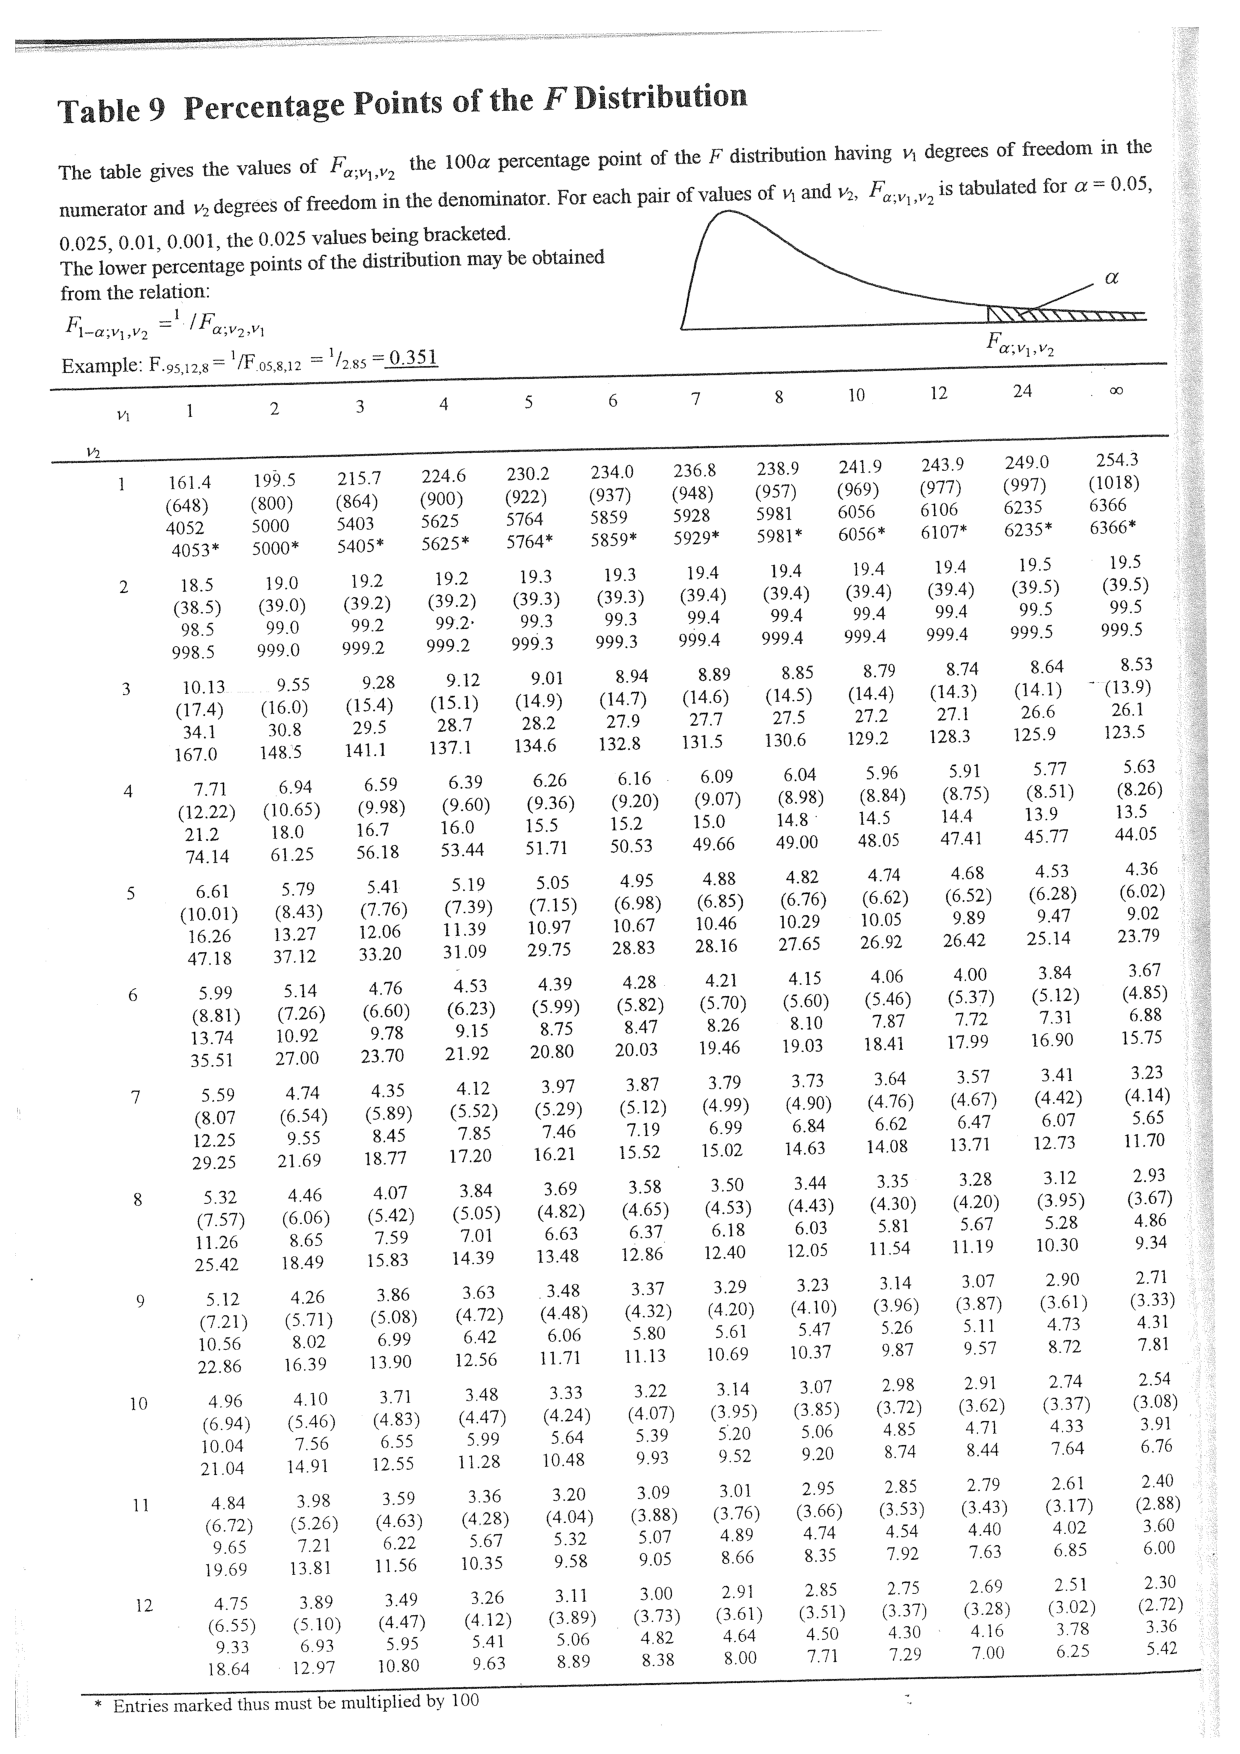
\includegraphics[width=1.1\textwidth, trim = 1cm 0.7cm 1cm 1cm, clip]{mdF}
\end{adjustwidth}

\newpage
\quad
\newpage

\section*{Answer Sheet\\[0.3cm]}

\subsection*{Name:\quad\underline{\hspace{11.45cm}}\\[0.3cm]}
\subsection*{ID Number:\quad\underline{\hspace{10cm}}\\[0.5cm]}

Enter your answers with an ``X' in the table below.\\[0.3cm]
Do not enter the ``X'' until you have made your \emph{final decision} to avoid scribbling out.\\[0.3cm]
\begin{large}
\begin{center}
\begin{tabular}{|c|c|c|c|c|}
\hline
&&&&\\[-0.4cm]
 & A & B & C & D \\
\hline
&&&&\\[-0.4cm]
Q1 &&&& \\
\hline
&&&&\\[-0.4cm]
Q2 &&&& \\
\hline
&&&&\\[-0.4cm]
Q3 &&&& \\
\hline
&&&&\\[-0.4cm]
Q4 &&&& \\
\hline
&&&&\\[-0.4cm]
Q5 &&&& \\
\hline
\multicolumn{5}{c}{}\\[-0.3cm]
\hline
&&&&\\[-0.4cm]
Q6 &&&& \\
\hline
&&&&\\[-0.4cm]
Q7 &&&& \\
\hline
&&&&\\[-0.4cm]
Q8 &&&& \\
\hline
&&&&\\[-0.4cm]
Q9 &&&& \\
\hline
&&&&\\[-0.4cm]
Q10 &&&& \\
\hline
\multicolumn{5}{c}{}\\[-0.3cm]
\hline
&&&&\\[-0.4cm]
Q11 &&&& \\
\hline
&&&&\\[-0.4cm]
Q12 &&&& \\
\hline
&&&&\\[-0.4cm]
Q13 &&&& \\
\hline
&&&&\\[-0.4cm]
Q14 &&&& \\
\hline
&&&&\\[-0.4cm]
Q15 &&&& \\
\hline
\end{tabular}
\end{center}
\end{large}


\end{document} 